\documentclass[10pt,oneside,a4paper]{article}

% DO NOT add \usepackage commands here.  Place any custom commands
% into your SV work files.  Anything in the template directory is
% likely to be overwritten!

\usepackage{fancyhdr}

\usepackage{lastpage}       % ``n of m'' page numbering
\usepackage{lscape}         % Makes landscape easier

\usepackage{verbatim}       % Verbatim blocks
\usepackage{listings}       % Source code listings
\usepackage{graphicx}
\usepackage{float}
\usepackage{epsfig}         % Embed encapsulated postscript
\usepackage{array}          % Array environment
\usepackage{qrcode}         % QR codes
\usepackage{enumitem}       % Required by Tom Johnson's exam question header

\usepackage{hhline}         % Horizontal lines in tables
\usepackage{siunitx}        % Correct spacing of units
\usepackage{amsmath}        % American Mathematical Society
\usepackage{amssymb}        % Maths symbols
\usepackage{amsthm}         % Theorems

\usepackage{ifthen}         % Conditional processing in tex

\usepackage[top=3cm,
            bottom=3cm,
            inner=2cm,
            outer=5cm]{geometry}

% PDF metadata + URL formatting
\usepackage[
            pdfauthor={\studentname},
            pdftitle={\svcourse, SV \svnumber},
            pdfsubject={},
            pdfkeywords={9d2547b00aba40b58fa0378774f72ee6},
            pdfproducer={},
            pdfcreator={},
            hidelinks]{hyperref}

\renewcommand{\headrulewidth}{0.4pt}
\renewcommand{\footrulewidth}{0.4pt}
\fancyheadoffset[LO,LE,RO,RE]{0pt}
\fancyfootoffset[LO,LE,RO,RE]{0pt}
\pagestyle{fancy}
\fancyhead{}
\fancyhead[LO,RE]{{\bfseries \studentname}\\\studentemail}
\fancyhead[RO,LE]{{\bfseries \svcourse, SV~\svnumber}\\\svdate\ \svtime, \svvenue}
\fancyfoot{}
\fancyfoot[LO,RE]{For: \svrname}
\fancyfoot[RO,LE]{\today\hspace{1cm}\thepage\ / \pageref{LastPage}}
\fancyfoot[C]{\qrcode[height=0.8cm]{\svuploadkey}}
\setlength{\headheight}{22.55pt}


\ifthenelse{\equal{\jkfside}{oneside}}{

 \ifthenelse{\equal{\jkfhanded}{left}}{
  % 1. Left-handed marker, one-sided printing or e-marking, use oneside and...
  \evensidemargin=\oddsidemargin
  \oddsidemargin=73pt
  \setlength{\marginparwidth}{111pt}
  \setlength{\marginparsep}{-\marginparsep}
  \addtolength{\marginparsep}{-\textwidth}
  \addtolength{\marginparsep}{-\marginparwidth}
 }{
  % 2. Right-handed marker, one-sided printing or e-marking, use oneside.
  \setlength{\marginparwidth}{111pt}
 }

}{
 % 3. Alternating margins, two-sided printing, use twoside.
}


\setlength{\parindent}{0em}
\addtolength{\parskip}{1ex}

% Exam question headings, labels and sensible layout (courtesy of Tom Johnson)
\setlist{parsep=\parskip, listparindent=\parindent}
\newcommand{\examhead}[3]{\section{#1 Paper #2 Question #3}}
\newenvironment{examquestion}[3]{
\examhead{#1}{#2}{#3}\setlist[enumerate, 1]{label=(\alph*)}\setlist[enumerate, 2]{label=(\roman*)}
\marginpar{\href{https://www.cl.cam.ac.uk/teaching/exams/pastpapers/y#1p#2q#3.pdf}{\qrcode{https://www.cl.cam.ac.uk/teaching/exams/pastpapers/y#1p#2q#3.pdf}}}
\marginpar{\footnotesize \href{https://www.cl.cam.ac.uk/teaching/exams/pastpapers/y#1p#2q#3.pdf}{https://www.cl.cam.ac.uk/\\teaching/exams/pastpapers/\\y#1p#2q#3.pdf}}
}{}


\fancyhead[RO,LE]{{\bfseries NST Maths, SV~17}\\ 28-05-2022 12:00, Video Link}

\usepackage{physics}
\usepackage{pdfpages}
\usepackage{graphicx}
\usepackage{float}

\begin{document}

\begin{enumerate}

\item Let $\psi = X(x)Y(y)$ for some functions $X$, $Y$.

\[
\begin{split}
\pdv[2]{\psi}{x} + \pdv[2]{\psi}{y} &= 0 \Longrightarrow \\
X^{(2)}(x)Y(y) + X(x)Y^{(2)}(y) &= 0 \\
\frac{X^{(2)}(x)}{X(x)} &= -\frac{Y^{(2)}(y)}{Y(y)} \\
\end{split}
\]
Since they are equal, the result of both of these must be independent of $x$ and $y$.

This forms two ordinary differential equations:
\begin{align*}
X^{(2)}(x) - kX(x) &= 0 & Y^{(2)}(y) + kY(x) &= 0 \\
\end{align*}

Which leads us to three possible equations dependent on the values of $k$:
\[
\psi =
\begin{cases}
(Ax + B)(Cy + D) & \text{ if } k = 0 \\
(Ae^{\lambda x} + Be^{-\lambda x})C\sin(\lambda y + \phi) & \text{ if } k > 0 \text{ where } k = \lambda^2 \text{
with } 0 \leq \psi < \pi \\
A\sin(\lambda x + \phi)(Ce^{\lambda y} + De^{-\lambda y}) & \text{ if } k < 0 \text{ where } k = - \lambda^2 \text{
with } 0 \leq \psi < \pi \\
\end{cases}
\]

Note that in cases $k = 0$ and $k < 0$, the function $Y$ is not cyclic -- meaning that the criteria $\psi(x, 0) =
\psi(x, a)$. So $k > 0$ must be true.

Using the boundary condition $\psi(x, 0) = 0$:

\[
\begin{split}
(Ae^{\lambda x} + Be^{-\lambda x})C\sin(0 + \phi) &= 0 \Longrightarrow \\
\sin(\phi) &= 0 \Longrightarrow \\
\psi &= 0 \\
\end{split}
\]

Using the boundary condition $\psi(x, a) = 0$:

\[
\begin{split}
(Ae^{\lambda x} + Be^{-\lambda x})C\sin(\lambda a) &= 0 \Longrightarrow \\
\sin(\lambda a) &= 0 \Longrightarrow \\
\lambda a &= n\pi \Longrightarrow \\
\lambda &= \frac{n\pi}{a} \\
\end{split}
\]

Notice that $\lim_{x \rightarrow \infty} \psi(x, y) = 0$. So $A = 0$.

Using the principle of superposition and the boundary condition $\psi(0, y) = \sin\left(\frac{\pi y}{a}\right) + 2\sin\left( \frac{\pi y}{a}
\right)$:
\[
\begin{split}
\psi &= \sum^{\infty}_{n=0} B_{n}C_n e^{-\frac{\pi n}{a} x} \sin\left(\frac{\pi n}{a} y\right) \\
\psi(0, y) &= \sum^{\infty}_{n=0} K_n \sin\left(\frac{\pi n}{a} y\right) \\
\sin\left(\frac{\pi y}{a}\right) + 2\sin\left( \frac{\pi y}{a}
\right) &= \sum^{\infty}_{n=0} K_n \sin\left(\frac{\pi n}{a} y\right) \Longrightarrow \\
K_n &= \begin{cases}
1 & \text{ if } n = 1 \\
2 & \text{ if } n = 2 \\
0 & \text{ otherwise } \\
\end{cases} \\
\psi(x, y) &= e^{-\frac{\pi x}{a}}\sin\left( \frac{\pi y}{a} \right) +
2 e^{-\frac{2\pi x}{a}}\sin\left( \frac{2\pi y}{a} \right)
\end{split}
\]

\item
\[
\pdv[2]{\phi}{x} + \pdv[2]{\phi}{y} = 0
\]

Using the method of separation of variables:
\[
\phi =
\begin{cases}
(ax + b)(cy + d) \\
(Ae^{\lambda x} + Be^{-\lambda x})C\sin(\lambda y + \theta) \\
A\sin(\lambda x + \theta)(Ce^{\lambda y} + De^{-\lambda y}) \\
\end{cases}
\]
Since $\phi$ is periodic with $x$, we can conclude that case 3 is the correct
case. Note that since $x$ is periodic with period $\pi$ and $\phi(0, y) = 0$,
we can derive that $\theta = 0$ and $\exists n \in \mathbb{N}. \lambda = n$.
By the principle of superposition, we can therefore form:
\[
\phi = \sum^{\infty}_{n=1}  A_n\sin(n x)(C_n e^{n y} + D_n e^{-n y}) \\
\]
Noting the constraint $\phi(x, 0) = 0$:
\[
C_n + D_n = 0 \Longrightarrow D_n = -C_n
\]
We now have the expression:
\[
\phi = \sum^{\infty}_{n=1} A_n C_n\sin(n x)(e^{n y} - e^{-n y}) \\
\]
Replacing $A_n C_n$ with $K_n$, equating with $\phi(x, b)$ and then using orthogonality gives:
\[
\begin{split}
\phi(x, y) &= \sum^{\infty}_{n=1} K_n\sin(n x)(e^{n y} - e^{-n y}) \\
\int^\pi_0 x(\pi - x)\sin(nx) dx &= K_n \int^{\pi}_0 \sin^2(n x) (e^{n b} - e^{-n b}) dx \\
K_n &= \frac{\left[ \frac{x^2}{n}\cos(nx) - \frac{2x}{n^2}\sin(nx) - \frac{2}{n^2}\cos(nx) - \frac{\pi x}{n}\cos(nx)
+ \frac{\pi}{n^2}\sin(nx) \right]^\pi_0}{(e^{n b} - e^{-n b})\left[ \frac{1}{2}x - \frac{1}{4n}\sin(2nx) \right]^\pi_0}\\
K_n &= \frac{\frac{\pi^2}{n}\cos(n\pi) - \frac{2}{n^2}\cos(n\pi) - \frac{\pi^2}{n}\cos(n\pi) + \frac{2}{n^2}}{(e^{n b} - e^{-n
 b})\frac{1}{2}\pi} \\
K_n &= \frac{\frac{2}{n^2}(1 - (-1)^n)}{(e^{n b} - e^{-n b})\frac{1}{2}\pi} \\
K_n &= \frac{4(1 - (-1)^n)}{n^2 \pi (e^{n b} - e^{-n b})} \\
\end{split}
\]
So:
\[
\phi(x, y) = \sum^{\infty}_{n=1} \frac{4(1 - (-1)^n)}{n^2 \pi (e^{n b} - e^{-n b})} \sin(n x)(e^{n y} - e^{-n y}) \\
\]

\item

\[
\begin{split}
y(x, t) &= f(x - ct) + g(x + ct) \Longrightarrow \\
\pdv[2]{y}{t} &= c^2 f^{(2)}(x - ct) + c^2 g^{(2)}(x + ct) \\
\pdv[2]{y}{x} &= f^{(2)}(x - ct) + g^{(2)}(x + ct) \\
\pdv[2]{y}{x} &= \frac{1}{c^2}\left( c^2 f^{(2)}(x - ct) + c^2 g^{(2)}(x + ct) \right) \\
\pdv[2]{y}{x} &= \frac{1}{c^2} \pdv[2]{y}{t} \text{ as required } \\
\end{split}
\]

Since this expression holds for all $f, g$, consider the case $f(z) = g(z) = \frac{1}{2(1 + z^2)}$.
This gives the solution:
\[
y(x, t) = \frac{1}{2(1 + (x + ct)^2)} + \frac{1}{2(1 + (x - ct)^2)} \\
\]

\begin{figure}[H]
\centering
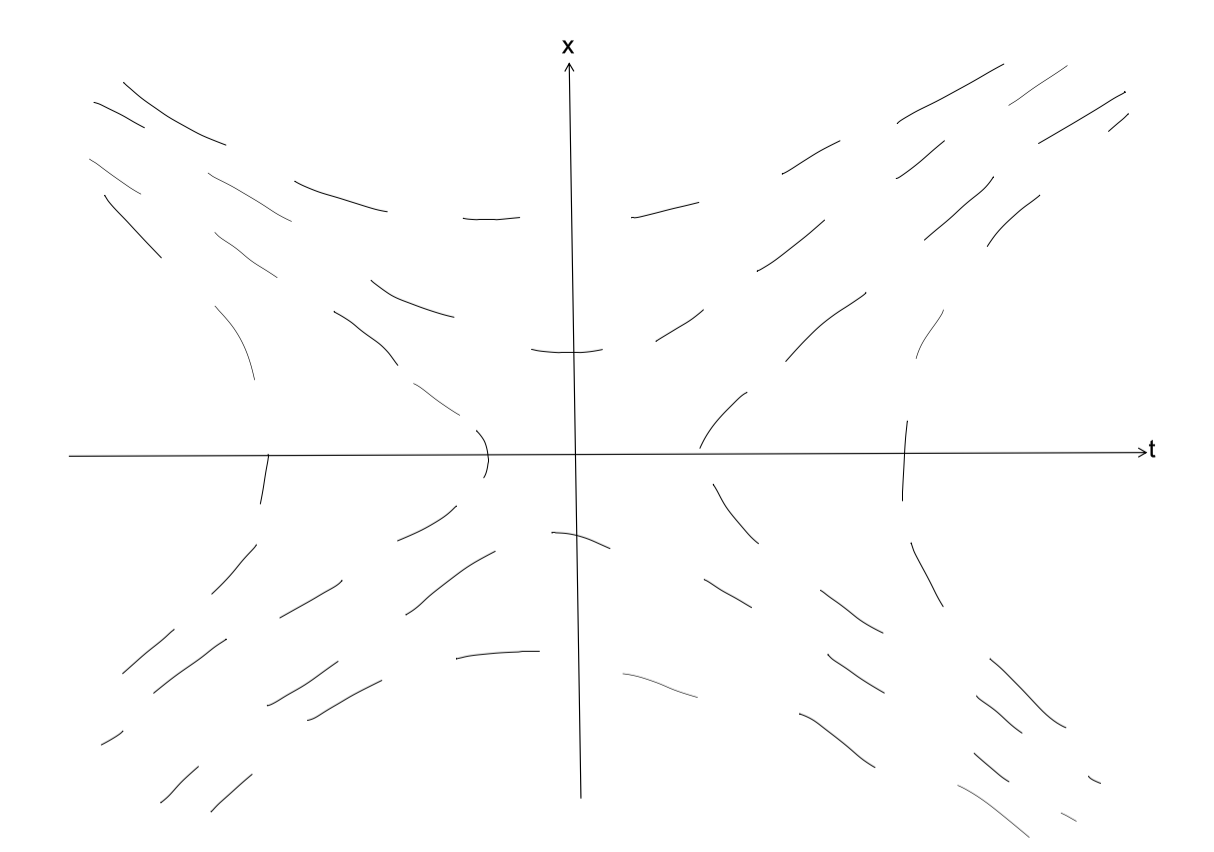
\includegraphics[width=\textwidth]{./diagramq3}
\end{figure}

\item
Since $y$ solves the wave equation, the solution is of the form $y = f(x + ct) + g(x - ct)$.

Let $f_n(u) = g_n(u) = A\sin\left(\frac{2n\pi u}{L}\right) + B\cos\left(\frac{2n\pi u}{L}\right)$. Since $f(x, 0)$ is
an even function, the sin terms must all be zero. Using the principle of superposition (and
knowing that the mean value of $y(x, 0)$ is $\frac{v}{2}$)
\[
\begin{split}
y &= \frac{v}{2} + \sum^\infty_{n=1} A\cos\left(\frac{2n\pi}{L}(x + ct)\right) + A\cos\left(\frac{2n\pi}{L}(x - ct)
\right) \\
y &= \frac{v}{2} + \sum^\infty_{n=1} 2A\cos\left(\frac{2n\pi x}{L}\right)\cos\left(\frac{2n\pi ct}{L}\right) \\
y(x, 0) &= \frac{v}{2} + \sum^\infty_{n=1} 2A\cos\left( \frac{2n\pi x}{L} \right) \\
\int^{L}_{0} y(x, 0)\cos\left( \frac{2n\pi x}{L} \right) \dd{x} &= \int^{L}_{0} 2A\cos^2\left( \frac{2n\pi x}{L}
\right) \dd{x} \\
\int^{\frac{3L}{4}}_{\frac{L}{4}} v\cos\left( \frac{2n\pi x}{L} \right) \dd{x} &= A\int^{L}_{0} \cos\left(
\frac{4n\pi x}{L}\right) + 1\dd{x} \\
\frac{Lv}{2n\pi}\left[ \sin\left( \frac{2n\pi x}{L} \right) \right]^{\frac{3L}{4}}_{\frac{L}{4}} &=
\frac{AL}{4n\pi}\left[ \sin\left( \frac{4n\pi x}{L} \right) + x \right]^L_0 \\
\frac{Lv}{2n\pi}\left( \sin \frac{3n\pi}{2} - \sin \frac{n\pi}{2} \right) &= \frac{AL^2}{4n\pi} \\
\frac{Lv(1 - (-1)^n)}{2n\pi} &= \frac{AL^2}{4n\pi} \\
A &= \frac{2v(1 - (-1)^n)}{L} \\
\end{split}
\]

So the expression for $y(x, t)$ is:
\[
y(x, t) = \frac{v}{2} + \frac{4v}{L}\sum^\infty_{n=1} (1 - (-1)^n)\cos\left(\frac{2n\pi x}{L}\right)\cos\left
(\frac{2n\pi ct}{L}\right) \\
\]

\item

\[
\pdv[2]{\Theta}{x} = \frac{1}{\kappa}\pdv{\Theta}{t} \\
\]

Let $\Theta = X(x)T(t)$.
\begin{align*}
\pdv[2]{\Theta}{x} &= X^{(2)}(x)T(t) & \pdv{\Theta}{t} &= X(x)T^{(1)}(t)
\end{align*}

Substituting this into the diffusion equation gives:
\[
\begin{split}
X^{(2)}(x)T(t) &= \frac{1}{\kappa} X(x)T^{(1)}(t) \\
\frac{X^{(2)}(x)}{X(x)} &= \frac{T^{(1)}(t)}{\kappa T(t)} \\
\end{split}
\]
Since these functions are equal to each other, they must both be independent of
$x$ and $t$ and so must be equal to some constant. This leads to several solutions.
Since we know that the solution for $t=0$ is given by a sum of $\sin$ in $x$, we know that
the constant is negative. Let it be $-\lambda^2$.

\[
\begin{split}
\frac{X^{(2)}(x)}{X(x)} &= -\lambda^2 \\
X^{(2)}(x) + \lambda^{2}X(x) &= 0 \\
X(x) &= A\cos(\lambda x) + B\sin(\lambda x) \\
\end{split}
\]
Since we have the boundary condition that for $\Theta(x, 0)$ is a sum of $\sin$,
the $A$ must be zero.

\[
\begin{split}
\frac{T^{(1)}(t)}{\kappa T(t)} &= -\lambda^2 \\
T^{(1)}(t) &= - \kappa\lambda^{2}T(t) \\
T(t) &= Ce^{-\kappa\lambda^2 t} \\
\end{split}
\]

Letting $AC = b_n$ and substituting $\lambda = \frac{n\pi}{l}$ for arbitrary $n$, $\Theta(x, t) = a \sin\left(\frac{n\pi x}{l}\right)
e^{-\frac{n^2\pi^2 \kappa x}{l^2} t} $ is a solution
the differential equation

By the principle of superposition:
\[
\Theta(x, t) = \sum^{\infty}_{n=1} b_n \sin\left( \frac{n\pi x}{l} \right)e^{-\frac{n^2\pi^2 \kappa t}{l^2}} \\
\]

So the required expression is both a solution to the diffusion equation and
satisfies the boundary conditions.

\item

\[
\begin{split}
u(r, t) &= \frac{A}{t}e^{-\frac{r^2}{4\kappa t}} \\
\pdv{u}{r} &= -\frac{Ar}{2\kappa t^2}e^{-\frac{r^2}{4\kappa t}} \\
r\pdv{u}{r} &= -\frac{Ar^2}{2\kappa t^2}e^{-\frac{r^2}{4\kappa t}} \\
\pdv{r}\left( r\pdv{u}{r} \right) &= \left(\frac{Ar^3}{4\kappa^2 t^3} - \frac{Ar}{\kappa t^2}\right)
e^{-\frac{r^2}{4\kappa t}} \\
\frac{1}{r}\pdv{r}\left( r\pdv{u}{r} \right) &= \left(\frac{Ar^2}{4\kappa^2 t^3} - \frac{A}{\kappa t^2}\right)
e^{-\frac{r^2}{4\kappa t}} \\
\end{split}
\]

\[
\begin{split}
u(r, t) &= \frac{A}{t}e^{-\frac{r^2}{4\kappa t}} \\
\pdv{u}{t} &= \left( \frac{Ar^2}{4\kappa t3} - \frac{A}{t^2}\right)e^{-\frac{r^2}{4\kappa t}} \\
\frac{1}{\kappa} \pdv{u}{t} &= \left( \frac{Ar^2}{4\kappa t3} - \frac{A}{t^2} \right)e^{-\frac{r^2}{4\kappa
t}} \\
\frac{1}{\kappa} \pdv{u}{t} &= \frac{1}{r}\pdv{r}\left( r\pdv{u}{r} \right) \\
\end{split}
\]

So $u(r, t)$ is a solution to the partial differential equation.

The total number of drunks $N$ is given by the integral over $r$ at a given time $t$ (assuming
the drunks don't sober up).

\[
\begin{split}
N &= \int^{2\pi}_{0}\dd{\theta} \int^{\infty}_{0} \frac{A}{t}e^{-\frac{r^2}{4\kappa t}} r\dd{r} \\
&= 2\pi \left[ -2A\kappa e^{-\frac{r^2}{4\kappa t}} \right]^{\infty}_0 \\
&= 2\pi \times 2A\kappa \\
&= 4\pi A \kappa \\
\end{split}
\]

Consider the density of drunks at distance $R$. We can find the maximum of this by differentiating
with respect to $t$.

\[
\begin{split}
u(R, t) &= \frac{A}{t}e^{-\frac{R^2}{4\kappa t}} \\
\pdv{u}{t} &= \left( \frac{AR^2}{4\kappa t^3} - \frac{A}{t^2}\right)e^{-\frac{R^2}{4\kappa t}} \\
0 &= \frac{AR^2}{4\kappa t^3} - \frac{A}{t^2} \\
0 &= R^2 - 4\kappa t \\
t &= \frac{R^2}{4\kappa} \\
\end{split}
\]
So the maximum density of drunks at distance $R$ from the pub happens at $t = \frac{N}{AR^2 \pi}$. Substituting
this into the original equation gives the maximum density of drunks at distance $R$ is:
\[
\begin{split}
u(R, t)_{\max} &= \frac{4A\kappa}{R^2} e^{-\frac{4\kappa R^2}{4\kappa R^2}} \\
&= \frac{4\pi A\kappa}{R^2 \pi}e^{-1} \\
&= \frac{N}{R^2 \pi e}
\end{split}
\]

\end{enumerate}

\end{document}